%!TEX root = ./cikm2016.tex

\section{Knowledge Population}
\label{sec:exp2}

In this section, we show results of incremental knowledge population task using Thomson sampling on the three datasets.
Additional verification on the Thompson sampling with synthetic datasets is also provided in Appendix \ref{sec:thompson_synthetic}.
%\rev{These experiments compare exploitation and exploration
% with exploitation only algorithms, and also show how the compositional model
%improves the entity embedding upon the non-compositional models. }
%%LX: second sentence can be cut if we need space.

\begin{figure*}[t]
	\centering

	\subfigure[KINSHIP]{
	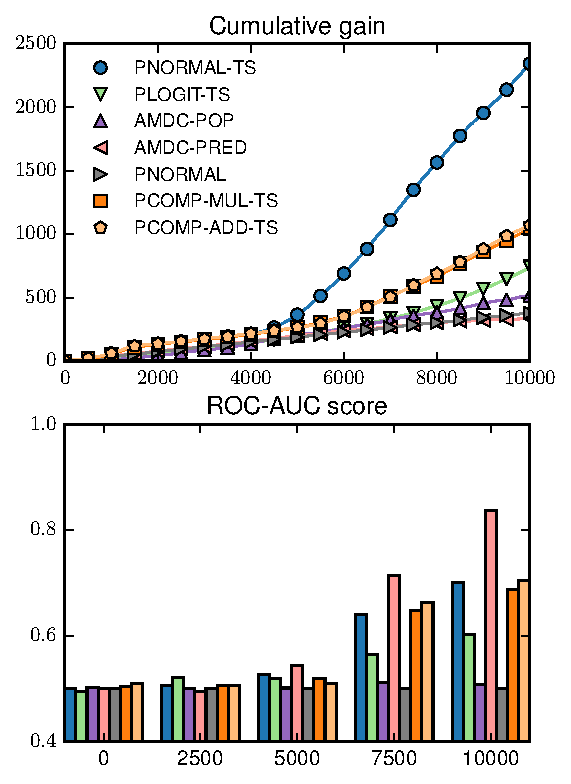
\includegraphics[width=0.295\linewidth]{images/thompson_kinship_mcmc_vertical_line.pdf}
	}
	\subfigure[UMLS]{
	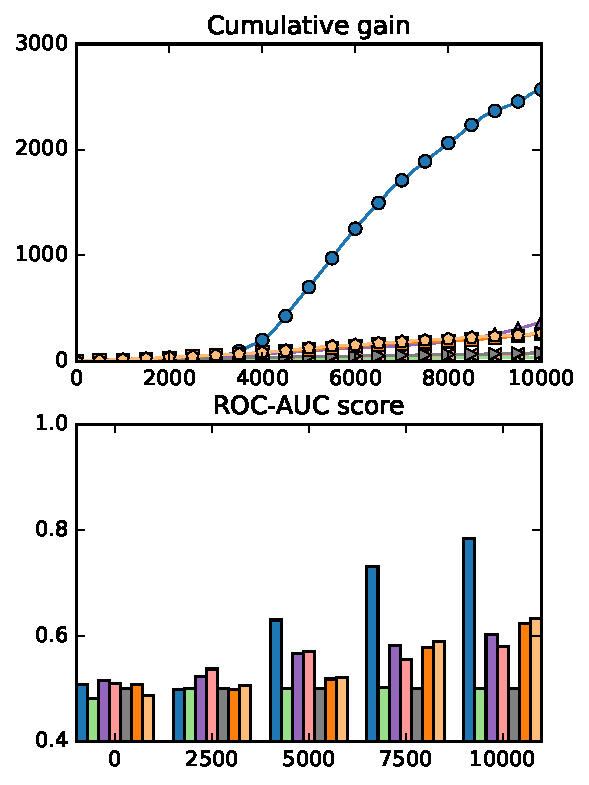
\includegraphics[width=0.295\linewidth]{images/thompson_umls_mcmc_vertical_line.pdf}
	}
	\subfigure[NATION]{
	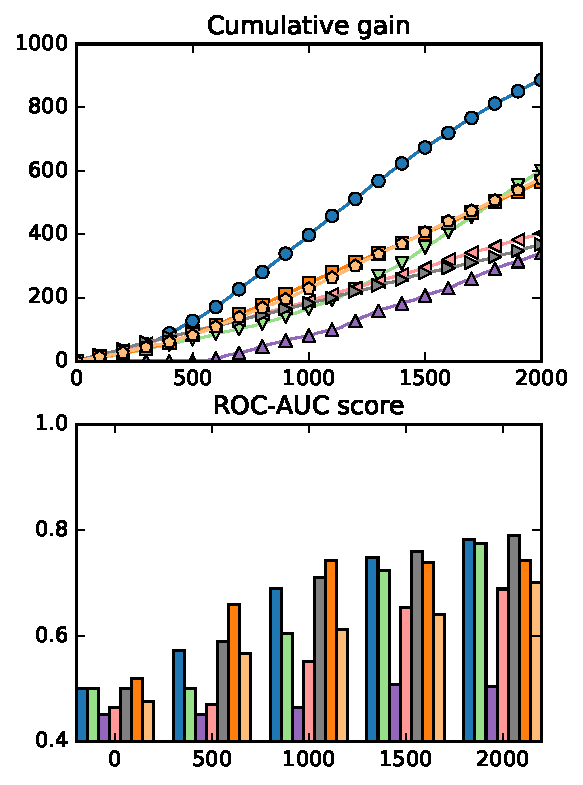
\includegraphics[width=0.295\linewidth]{images/thompson_nation_mcmc_vertical_line.pdf}
	}
	\caption{\label{fig:vs_greedy} The cumulative gain and ROC-AUC score of the Thompson sampling with passive learning and  AMDC models. Thompson sampling with PRESCAL (\textsc{PNORMAL-TS}) model achieves the highest cumulative gain to compare with the other models and shows comparable performance on ROC-AUC scores.}
\end{figure*}

% \subsection{Thompson sampling on real datasets}
%
% Next, we evaluate particle Thompson sampling for both compositional and non-compositional models on real datasets.

\textbf{Experimental settings}:
We compare the Thompson sampling models with \textsc{Amdc} models, and \textsc{Prescal} for passive learning.
\textsc{Amdc} model has been proposed to achieve two different active learning goals, constructing a predictive
model and maximising the valid triples in a knowledge base, with two different querying strategies
~\cite{kajino2015active}.
\textsc{Amdc-pred} is a predictive model construction strategy and chooses a triple which is the most ambiguous (close to the decision boundary) at each time $t$.
\textsc{Amdc-pop} is a population strategy which aims to maximise the number of valid triples in a knowledge base, choosing a triple with the highest expected value at each time.
To train all models we only use the observed triples up to the current time.
For the passive learning with \textsc{Prescal}, we generate a random sample at each time period.
For the particle Thompson sampling models, we set variance parameter $\sigma_e$ and $\sigma_r$ to 1, $\sigma_x$ to 0.1, and vary $\sigma_c$ from 1 to 100.

We leave 30 \% of triples as a test set to measure test error.
At each time period, each model chooses one triple to query,
if the selected triple is in the test set then we choose the next highest expected triple that is not in the test set.
All models start from zero observation.
After every query, a model obtains a label of the queried triple from an oracle,
then the model updates the parameters.

\textbf{Evaluation metric}: We use two different evaluation metrics, the cumulative gain and ROC-AUC score,
for the performance comparison. The goal of the Thompson sampling is to maximise the knowledge
population through the balanced querying strategy between exploration and exploitation.
To measure how many triples are obtained through the querying stage, we compute the cumulative
gain which is the number of valid triple obtained up to time $t$. Additionally, we compute the ROC-AUC score on
the test set to understand how this balanced querying strategy results in making a predictive model.

\textbf{Exploitation and exploration}:
Figure \ref{fig:vs_greedy} shows
the cumulative gains and ROC-AUC scores of the Thompson sampling on three real datasets. The model names with suffix \textsc{-ts} represent the models adopting the Thompson sampling strategy.
\textsc{Pnormal-ts} performs better than other baseline models for the cumulative gain, and shows comparable result for the ROC-AUC scores. Both compositional models perform worse than \textsc{Pnormal-ts} across all datasets.

In the original \textsc{Amdc} \cite{kajino2015active}, \textsc{Amdc-pop} model obtains more
valid triples than \textsc{Amdc-pred}, and \textsc{Amdc-pred} shows high ROC-AUC scores than \textsc{Amdc-pop}.
In our experiment, however, \textsc{Amdc-pop} shows comparable cumulative gain to \textsc{Amdc-pred}
and even worse than \textsc{Amdc-pred} for the UMLS. We conjecture the initial observation and query size results in the different performances: in the original experiment, the model starts
from a small set of training data, and the query size was 1,000 for KINSHIP and UMLS. With larger query size, the model focuses on exploit and takes advantages, whereas in our experiment, we start from zero observation and query one triple at each time, which makes the model hard to exploit. This result shows
the importance of balancing between exploitation and exploration.

\eat{
\begin{figure}[t]
	\centering

	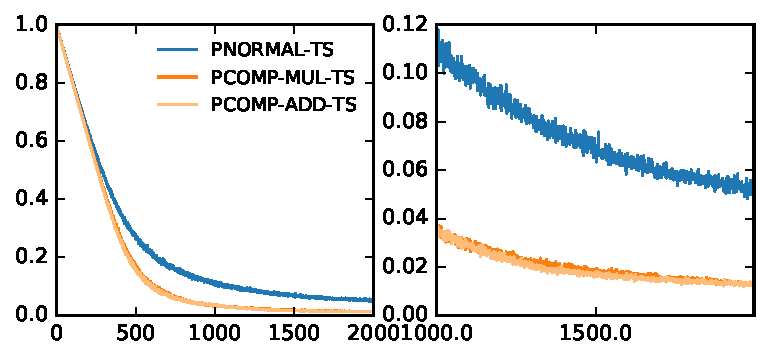
\includegraphics[width=0.9\linewidth]{images/posterior_variance_trace_kinship.pdf}

	\caption{\label{fig:pos_var} Trace plot of mean posterior variance of the non-compositional model and compositional models. Y-axis denotes the average posterior covariance, and X-axis denotes the number of queries. The second plot magnifies the first plot.}
\end{figure}
}

We note that the compositional model performs worse than the non-compositional models,
especially than \textsc{Pnormal-ts}.
This is counter-intuitive to our general understanding where
the model that performs well in the predictive task also shows
a better performance in the active learning.

\eat{
Of course, we also emphasise the difference between two experiments;
the goal of incremental population is to maximise the number of triples
whereas the goal of knowledge completion in Section \ref{sec:exp1} is to maximise
the predictive performance. Nevertheless, the compositional models do not outperform
\textsc{Pnormal-ts} in the active learning.
This result can be partially understood in terms of the balance between
exploration-exploitation. Figure \ref{fig:pos_var} shows the average posterior variance of
the entity vectors. We compute the eigenvalues of posterior covariance matrix $\Lambda_i^{-1}$
and trace the average eigenvalues over the iterations.
As shown in the figure, the average variance of the compositional model shrinks much faster
than the \textsc{Pnormal-ts}. Because the exploration-exploitation of the Thompson sampling depends on the
posterior uncertainty, the fast shrinkage in the posterior variance may indicate the under
exploration of the model. This is predictable to a certain extent in the sense that one new triple with the compositional models induces multiple new
observations in the compositional triples, so the uncertainties of entities and
relations are measured less than those with non-compositional model. Most active
learning algorithms utilise model uncertainty, and hence a model with augmented
structures such as the relation compositions should be more careful about reflecting its uncertainty correctly.
}

\eat{If the samples of the compositional model follows the posterior
distribution, it may show the similar performance with the passive learning
scenario, but this assumption does not always hold since the active sampling
path does not correspond to the passive scenario. } %%LX: this looks like too much detail
\eat{
One possible explanation is
that the naive particle Thompson sampling may not capture the posterior of the
complex compositional structure, so the particle degenerates over time. Recent
 advances in sequential Monte Carlo may help to solve the problem\cite{gu2015neural,naesseth2014sequential,lindsten2014divide}.
We leave this for future work.
}
